\chapter{Quantum Many-Body Entanglement and Tensor Networks}

In session 6 we studied the magnetism of the Hubbard model of session 1 in full numerical detail. We
derived the Heisenberg model as the strong-coupling limit, we introduced Holstein-Primakoff magnons,
and we used the topological methods of sessions 3 and 4 for a third time, now for magnon bands. In
that session we also mentioned the Kitaev interaction as an important ingredient for quantum spin
liquids, and we mentioned materials such as herbertsmithite, where the local moments sit on a kagome
lattice and do not order even at zero temperature. That session ended with ``topological magnons,''
without a final summary. This was not a transition into the present session, since that session had
reached the end of its material, but the open topic is the one we continue with now. In contrast with a ferromagnet or an antiferromagnet, a quantum spin liquid does not
break time-reversal symmetry. Its spins keep fluctuating locally for any low temperature, and the
ground state is one large entangled object and not a simple pattern of arrows. All the tools that we
have built in this course so far fail for this kind of Hamiltonian. Mean-field theory, which we have
used since session 1, looks for an order parameter that breaks a symmetry, such as a nonzero
magnetization, a nonzero charge imbalance or a nonzero pairing amplitude. By definition, a quantum
spin liquid has none of these, so the self-consistent calculation has nothing to converge to and
gives back zero, which tells us nothing about the real ground state. The same problem appears in a
second family of materials, the fractional Chern insulators, where the interactions are again too
strong to be described by any effective single-particle model.

In this session we will build a tool that works directly in this regime and does not assume that a
symmetry is broken. This tool is tensor networks, and in particular matrix product states (MPS). This
method is well developed, and today it gives the best quantitative evidence for spin liquid physics on
the triangular and kagome lattices, which are the Hamiltonians mentioned in session 6. To get there,
we first point out something that was present in the last sessions without being said explicitly,
which is that fermionic and spin Hamiltonians describe the same physics in two languages, and the
link between them is the Jordan-Wigner transformation. Then we will ask a question which is not
``how do we diagonalize a huge matrix'' but ``how do we \emph{store} a many-body wave function in
the first place.'' To answer this question we will use entanglement and a quantity called the
entanglement entropy, and this is the main part of this session.

\section{Two regimes of many-body physics}

Let us go back to the general interacting Hamiltonian that we have used in the whole course,

\begin{equation}
H = \sum_{ij} t_{ij}\, c_i^\dagger c_j \;+\; \sum_{ijkl} V_{ijkl}\, c_i^\dagger c_j c_k^\dagger c_l.
\end{equation}

The kinetic term is free and can be solved exactly, and the interaction term in general cannot. In all
sessions so far we treated (7.1) in the same way. We decoupled the quartic term with mean field, we
replaced it with an effective bilinear Hamiltonian, and we looked at which symmetry is broken by the
resulting order parameter. This strategy defines what we can call \textbf{weakly correlated matter}.
In this sense, magnets, superconductors and charge density waves are all single-particle physics,
once we find the right symmetry-broken background.

In this session we are in the opposite regime, which is \textbf{strongly correlated matter}. Here the
interactions are so strong that no effective single-particle Hamiltonian gives the ground state, for
any choice of the decoupling. Quantum spin liquids and fractional Chern insulators are our two main
examples, and more generally, the same problem appears when we want an accurate phase diagram of a
truly interacting model. In both cases we cannot solve the problem with an ansatz for the broken
symmetry. Instead, we need something close to an exact numerical solution, or at least a controlled
approximation that does not assume symmetry breaking from the start. This is what tensor networks
give us.

\section{Fermions, spins and the Jordan-Wigner transformation}

Before we build the tool, let us point out something that was present in the last sessions without
being said explicitly. We have used two families of many-body Hamiltonians that look different. The
first family is the fermionic Hamiltonians of the form (7.1), with a general two-body interaction
$V_{ijkl}$, where density-density interactions are only a special case, which we used in sessions 1 to 5. The second family is the spin Hamiltonians, mainly the
Heisenberg model $H =
\sum_{ij} J_{ij}\, \mathbf{S}_i \cdot \mathbf{S}_j$, which we used for the magnons of session 6 and
which we use again in this session for quantum spin liquids. These are not two different topics. They
are the same physics written in two different languages, and in this section we make this
translation precise.

Let us first look at a single site. A spinless fermionic site has a local Hilbert space of dimension
two, empty or full, and a spin-1/2 site also has a local Hilbert space of dimension two, down or up.
The first guess is $c_i^\dagger \leftrightarrow S_i^+$ and $c_i \leftrightarrow S_i^-$, and on a
single site this guess is exactly right. However, it fails when we have more than one site, since
fermion operators on different sites anticommute, while spin operators on different sites
commute. As a result, the naive identification gives
the wrong relative signs between sites. To fix this, we add to each site an extra phase that depends
on the occupations. This phase is a ``string'' over all the sites to the left, chosen so that the
exchange of two fermions gives the minus sign that the spin operators do not have by themselves. This
mapping is called the \textbf{Jordan-Wigner transformation}, and it reads

\begin{equation}
S_i^+ = c_i^\dagger K_i, \qquad S_i^- = c_i K_i, \qquad S_i^z = n_i - \tfrac{1}{2}, \qquad
K_i = \exp\!\left(i\pi \sum_{j<i} n_j\right),
\end{equation}

where $n_j = c_j^\dagger c_j$ is the fermion number operator on site $j$. The string operator $K_i$
is built only from the occupation numbers to the left of site $i$. For this reason it commutes with
all local operators on sites $j \ge i$, and it counts, mod 2, how many fermions are to the left. We
can check directly that (7.2), built in this way, gives the full $SU(2)$ commutation algebra of
spin-1/2 operators on every site and between every pair of sites. For this check we only need the
fermionic anticommutation relations for $c_i,
c_i^\dagger$ and the string. In the lecture this is summarized as \emph{spin equals fermion times
string}, and this statement is correct. Figure~\ref{fig:s07:jwstring} shows what the string does. It
counts the fermions to the left of site $i$ and gives their parity, so a change of a single occupation
anywhere in that region changes the sign of $S_i^+$.

% Session 7 -- the Jordan-Wigner string: "spin equals fermion times string".
% Placement: sec. "Fermions and spins are the same physics", after equation (7.2).
%
% LAYOUT NOTE: pure TikZ, no axis, so canvas coordinates throughout. Occupations
% are passed through the \foreach as a style name plus an arrow direction, so the
% fermion row and the spin row can never disagree with each other.
\begin{aqmfigure}{fig:s07:jwstring}{Spin equals fermion times string. Site by site the dictionary is
trivial: an empty site is a down spin, an occupied site an up spin, $S^z_i = n_i - \tfrac12$. It is
the \emph{relative} signs between sites that the naive identification gets wrong, because fermion
operators on different sites anticommute while spin operators on different sites commute. The string
$K_i$ of (7.2) repairs exactly this: it contributes a factor $-1$ once for every fermion sitting to
the left of site $i$. The two chains drawn here differ only in the occupations to the left of the
marked site $i=6$, three fermions above and two below, and that parity alone flips the sign of
$S_6^+ = c_6^\dagger K_6$. The string is genuinely nonlocal, and what it carries is the fermionic
exchange sign that spins do not have on their own.}

\begin{tikzpicture}[x=1cm, y=1cm]

\def\sx{0.80}   % site spacing

% ============================ legend ========================================
\node[aqmsite] at (0.15,1.72) {};
\node[aqmlabsmall, anchor=west] at (0.34,1.72) {occupied, $n_j=1$\;$\equiv$\;spin $\uparrow$};
\node[aqmsiteopen] at (4.35,1.72) {};
\node[aqmlabsmall, anchor=west] at (4.54,1.72) {empty, $n_j=0$\;$\equiv$\;spin $\downarrow$};

% ============================ chain 1 =======================================
\begin{scope}[shift={(0,0)}]
  \draw[aqm, draw=aqmmuted, line width=\aqmthinwidth] (-0.35,0) -- ({\sx*7+0.35},0);
  \foreach \i/\st/\dy in {0/aqmsite/1, 1/aqmsiteopen/-1, 2/aqmsite/1, 3/aqmsite/1,
                          4/aqmsiteopen/-1, 5/aqmsiteopen/-1, 6/aqmsite/1, 7/aqmsiteopen/-1} {
    \draw[aqm, draw=black, -{Stealth[length=3.4pt,width=2.8pt]}]
      ({\sx*\i},{0.66-0.19*\dy}) -- ({\sx*\i},{0.66+0.19*\dy});
    \node[\st] at ({\sx*\i},0) {};
  }
  \foreach \i/\lab in {0/1, 1/2, 2/3, 3/4, 4/5, 5/6, 6/7, 7/8} {
    \node[aqmlabmuted, anchor=north] at ({\sx*\i},-0.16) {\lab};
  }
  \node[circle, draw=aqmaccent, line width=\aqmlinewidth, minimum size=13pt,
        inner sep=0pt] at ({\sx*5},0) {};
  \node[aqmlabsmall, text=aqmaccent, anchor=south] at ({\sx*5},1.02) {$i=6$};

  \draw[aqmbrace, draw=aqmaccent] ({\sx*4+0.26},-0.60) -- (-0.26,-0.60);
  \node[aqmlabsmall, anchor=north, align=center, text=aqmaccent] at ({\sx*2},-0.74)
    {string $K_6$: every site $j<i$};

  \node[aqmlab, anchor=north west, align=left] at ({\sx*7+0.70},0.42)
    {three fermions to the left\\[2pt]
     $K_6=e^{i\pi\cdot 3}=-1$\\[2pt]
     \textcolor{aqmbroken}{$S_6^+=c_6^\dagger K_6=-\,c_6^\dagger$}};
\end{scope}

% ============================ chain 2 =======================================
\begin{scope}[shift={(0,-2.45)}]
  \draw[aqm, draw=aqmmuted, line width=\aqmthinwidth] (-0.35,0) -- ({\sx*7+0.35},0);
  \foreach \i/\st/\dy in {0/aqmsite/1, 1/aqmsiteopen/-1, 2/aqmsiteopen/-1, 3/aqmsite/1,
                          4/aqmsiteopen/-1, 5/aqmsiteopen/-1, 6/aqmsite/1, 7/aqmsiteopen/-1} {
    \draw[aqm, draw=black, -{Stealth[length=3.4pt,width=2.8pt]}]
      ({\sx*\i},{0.66-0.19*\dy}) -- ({\sx*\i},{0.66+0.19*\dy});
    \node[\st] at ({\sx*\i},0) {};
  }
  \foreach \i/\lab in {0/1, 1/2, 2/3, 3/4, 4/5, 5/6, 6/7, 7/8} {
    \node[aqmlabmuted, anchor=north] at ({\sx*\i},-0.16) {\lab};
  }
  \node[circle, draw=aqmaccent, line width=\aqmlinewidth, minimum size=13pt,
        inner sep=0pt] at ({\sx*5},0) {};
  \node[aqmlabsmall, text=aqmaccent, anchor=south] at ({\sx*5},1.02) {$i=6$};

  \draw[aqmbrace, draw=aqmaccent] ({\sx*4+0.26},-0.60) -- (-0.26,-0.60);
  \node[aqmlabsmall, anchor=north, align=center, text=aqmaccent] at ({\sx*2},-0.74)
    {same string, one occupation changed};

  \node[aqmlab, anchor=north west, align=left] at ({\sx*7+0.70},0.42)
    {two fermions to the left\\[2pt]
     $K_6=e^{i\pi\cdot 2}=+1$\\[2pt]
     \textcolor{aqmaccent}{$S_6^+=c_6^\dagger K_6=+\,c_6^\dagger$}};
\end{scope}

\end{tikzpicture}

\end{aqmfigure}


This is the one explicit link in the course between the two languages that we have used. The
fermionic operators of sessions 1 to 5 and the spin operators of session 6 and, as we will see, of
session 8 are related by (7.2), and they are not only analogous to each other. It also explains a
practical choice that we make for the rest of this session. Since interacting fermionic Hamiltonians
and interacting spin Hamiltonians are mathematically equivalent, we can work only in the spin
representation from now on, and we will do so. The reason is that spin operators on different sites
commute, so there is no fermionic sign to keep track of when we cut the chain, and this makes the
counting of entanglement below clean.

\section{Storing the wave function as the main bottleneck}

Now that we use the language of spins, let us ask why a general interacting many-body Hamiltonian is
hard to solve. A first answer would be ``because the diagonalization of a huge matrix is slow,'' but
the main problem is more basic, and it is the \emph{storage} of the wave function.

Let us take the simplest nontrivial case, which is the antiferromagnetic Heisenberg dimer, $H =
\mathbf{S}_0\cdot
\mathbf{S}_1$ on two spin-1/2 sites. Its ground state is the unique singlet,

\begin{equation}
|\Psi\rangle = \frac{1}{\sqrt{2}}\left(|{\uparrow\downarrow}\rangle -
|{\downarrow\uparrow}\rangle\right),
\end{equation}

which is a state that does not break any symmetry, since the expectation value of every single-site
spin vanishes. As we will show below, it is also maximally entangled. The question of the whole
session is how this kind of state generalizes to a macroscopic system with many sites.

Let us write a general spin-1/2 wave function in the natural product basis, with one up or down label
$s_i$ per site.

\begin{equation}
|\Psi\rangle = \sum_{s_1,\dots,s_L} C(s_1,\dots,s_L)\, |s_1,\dots,s_L\rangle, \qquad
s_i \in \{\uparrow,\downarrow\}.
\end{equation}

For $L=2$ there are four basis states, up-up, up-down, down-up and down-down, so there are four
coefficients $C$, and the Hamiltonian is a $4\times4$ matrix. If we add one site, $L=3$, the number
doubles to eight. If we add one more site, $L=4$, it doubles again to sixteen. In general, the
dimension of the Hilbert space is $d = 2^L$, and this is also the number of coefficients
$C(s_1,\dots,s_L)$ that we need to write the ground state exactly. This exponential growth is the
main limitation. Even if we never build the full $2^L\times2^L$ Hamiltonian matrix, and we only
compute the matrix elements when we need them, we still have to store the $2^L$ coefficients of the
ground state once we have found it. This storage cost, and not the cost of the diagonalization, is
the real obstruction, and it is the most important point of the whole session. Tensor networks are
one answer to this storage problem. In the lecture, \textbf{neural network quantum states} are also
mentioned briefly as a second answer to the same problem, which comes from machine learning, but
this second tool is not developed in this session. In session 10 we will come back to neural network
quantum states in detail, from the point of view of machine learning. The material of this session is
only about the first answer, tensor networks, and in particular matrix product states.

\begin{notebookbox}{\texttt{session7.ipynb}, ``Energy of the Heisenberg model as a function of the system size'' (Core)}
In this exercise you compute the ground-state energy per site of the Heisenberg chain with exact
diagonalization, for growing system sizes. For this you use the \texttt{dmrgpy} library, which is new
in this session, together with
\texttt{pyqula}. You will see how fast exact diagonalization stops being possible, and this limit is
the $2^L$ scaling of (7.4) in a concrete calculation.
\end{notebookbox}

\section{The matrix product state ansatz}

The idea that solves this problem is very simple. Instead of storing $C(s_1,\dots,s_L)$ as one large
array of $2^L$ numbers, we write it as a product of matrices, with one matrix for each possible value
of each local spin.

\begin{equation}
C(s_1,s_2,\dots,s_L) \;\approx\; M^{s_1}_{1}\, M^{s_2}_{2}\, \cdots\, M^{s_L}_{L},
\end{equation}

Here each $M^{s_i}_i$ is an $M\times M$ matrix, except at the two ends of a finite open chain where it
is a vector, and $M$ is the \textbf{bond dimension}, which is a free parameter that we choose. For a
spin-1/2 chain there are two matrices per site, one for $s_i=\uparrow$ and one for
$s_i=\downarrow$. Therefore the total number of parameters of the state is proportional to $L\times
M^2$, which is linear in the system size, in strong contrast with the $2^L$ of the exact
representation (7.4). This is called the \textbf{matrix product state} (MPS) ansatz. At first sight,
it is only a choice, and one that looks rather arbitrary. In Sections 7.5 to 7.8 we will answer two
questions about it. First, why it is a \emph{good} choice. Second, what exactly it captures, and what it
does not capture, about the physical state.

We should know from the start that this is not a toy model. Today matrix product states give the most
accurate results for two of the central hard problems in quantum materials. The first one is the doped
two-dimensional Hubbard model with second-neighbor hopping, which is related to unconventional
superconductivity. The second one is the two-dimensional frustrated Heisenberg model on the triangular
and kagome lattices, and this is where the strongest numerical evidence for real quantum spin liquid
physics comes from, which is the herbertsmithite example of session 6. Both examples are shown as
labeled figure panels on slide 15 of the deck, with the titles ``Solving the 2D Hubbard model at
finite doping'' and ``Solving the 2D Heisenberg model in frustrated lattices.'' This shows that MPS
are a working tool for the strongly correlated regime, and not only a formal construction.

\section{Measuring entanglement with the entanglement entropy}

To see why (7.5) works, we need a quantitative measure of how entangled a many-body state is. Let us
split the system into two complementary parts, subsystem $A$ and subsystem $B$. A state is \textbf{not
entangled}, which is also called a product state, if it can be written as $|\Psi\rangle = |\psi_A\rangle
\otimes
|\psi_B\rangle$. Two examples are the state $|{\uparrow\downarrow}\rangle$ and a product of two
single-site states that are both polarized along $x$. The singlet (7.3) is the opposite case. It cannot
be written as a product of this form, and it is our main example of an \textbf{entangled} state.

To turn the question ``entangled or not'' into a number, we define the full density matrix $\rho =
|\Psi\rangle
\langle\Psi|$, and we trace out subsystem $B$. This gives the \textbf{reduced density matrix} of $A$,
$\rho_A =
\mathrm{Tr}_B\,\rho$. The \textbf{entanglement entropy} is then the von Neumann entropy of $\rho_A$,

\begin{equation}
S(\rho_A) = -\,\mathrm{Tr}\!\left(\rho_A \log \rho_A\right).
\end{equation}

If $|\Psi\rangle$ is a product state, $\rho_A = |\psi_A\rangle\langle\psi_A|$ is a projector of rank
one, so its only nonzero eigenvalue is $1$, and we directly get $S=0$. This means that there is no
entanglement and the entropy is zero, which is what we expect.

Let us now check (7.6) on the singlet (7.3). We write $\rho = |\Psi\rangle\langle\Psi|$ in the product
basis and trace over site $1$, which is our subsystem $B$, and we obtain

\begin{equation*}
\rho_A = \tfrac{1}{2}\,|{\uparrow}\rangle\langle{\uparrow}| + \tfrac{1}{2}\,
|{\downarrow}\rangle\langle{\downarrow}|,
\end{equation*}

which is a maximally mixed single-site density matrix, with two eigenvalues both equal to $1/2$. Then

\begin{equation}
S = -\left(\tfrac12\log\tfrac12 + \tfrac12\log\tfrac12\right) = \log 2.
\end{equation}

This is the maximum entanglement entropy that a single spin-1/2 can have, since a local Hilbert space
of dimension $d$ can have at most $\log d$. This is the meaning of the statement that the singlet is
``maximally entangled,'' since it uses all the capacity of the local Hilbert space for entanglement.

\section{Entanglement entropy of a solvable dimerized chain}

There are two exactly solvable models that show how (7.6)-(7.7) scale with the system size. They are
the key to the whole session, so let us go through them carefully.

Let us take a one-dimensional chain of spin-1/2's, but we couple the spins only in separate pairs. There
is an antiferromagnetic bond between sites $0$ and $1$, another one between $2$ and $3$, another one
between $4$ and $5$, and so on, and there is \emph{no} coupling between different pairs,

\begin{equation*}
H = \sum_n J\,\mathbf{S}_{2n}\cdot\mathbf{S}_{2n+1}.
\end{equation*}

This Hamiltonian is easy to solve exactly, because it is a sum of independent Heisenberg dimers. Its
ground state is therefore an exact tensor product of singlets, with one singlet per dimer bond,

\begin{equation}
|\Psi\rangle = |\text{singlet}\rangle_{01} \otimes |\text{singlet}\rangle_{23} \otimes
|\text{singlet}\rangle_{45} \otimes \cdots.
\end{equation}

Physically, this is a valence-bond product state, also called a dimer product state, which is the
simplest example of a gapped state with short-range entanglement, and not a spin liquid. The ground
state does not break any symmetry of this Hamiltonian, and it is separated from the lowest triplet excitation by a large gap, which is the
singlet-triplet splitting of a single dimer. For this reason it is as far from criticality as a spin
model can be.

Now we divide the chain into two parts and ask for the entanglement entropy. Since (7.8) is a tensor
product over separate bonds, the reduced density matrix $\rho_A$ factorizes bond by bond. A dimer that
is fully inside $A$, or fully inside $B$, gives a pure state in $\rho_A$, and therefore it gives
exactly zero to $S$, with the same argument as for the product state in Section 7.5. The only bonds
that contribute are the ones that are cut by the boundary between the two parts. Each cut bond gives
the single-dimer result (7.7), $\log 2$, since tracing out one half of a singlet always leaves the same
maximally mixed single-site density matrix, regardless of what happens in the rest of the chain. So if
the boundary cuts $n_\text{cut}$ bonds, $S = n_\text{cut} \log 2$.

Let us take a small subsystem $A$ whose two ends cut through two dimers, one on each side. Then two
singlet bonds cross the boundary, so $S = 2\log 2$. Let us now take a much larger subsystem $A$, with
a width of many dimers, whose ends again cut through one dimer each. The boundary still crosses only
two singlet bonds, the ones at its two edges, so we get again $S = 2\log 2$,
with no change. \textbf{The entanglement entropy of this state does not grow with the size of the
subsystem}. It is fully determined by the two points where the one-dimensional boundary is, for any
distance between these two points.

\section{Two dimensions and the area law}

Let us now do the same construction in one more dimension. We take a two-dimensional lattice and we
group the sites into separate clusters of four sites, called tetramers, instead of pairs. The sites
inside a cluster are coupled, but different clusters are not coupled, so the ground state is again an
exact tensor product, now of tetramer ground states instead of dimer singlets. The same factorization
argument applies. A cluster fully inside $A$ or fully inside $B$ gives nothing, and only the clusters
that cross the boundary between the two parts contribute to $S$.

The only difference is geometric. Let us compare a small region $A$, whose boundary cuts eight bonds,
with a much larger region $A'$, whose longer boundary cuts many more bonds. Since the entropy again
gets one contribution per cut bond, $S$ is now set by the \emph{length of the boundary}. In two
dimensions this length grows when the subsystem grows. This is different from the 1D case of
Section 7.6, where the boundary was always two points for any size of the subsystem. This is the
central contrast. \textbf{In one dimension the entanglement entropy of a gapped ground state
saturates}, and it does not depend on the size of the subsystem. \textbf{In two or more dimensions it
grows with the size of the boundary}, $S_A \sim
L_A \sim \partial A$ and $S_{A'} \sim L_{A'} \sim \partial A'$, so $S_{A'} > S_A$ for the larger region.
Figure~\ref{fig:s07:arealaw} shows the two cases next to each other, with the cut bonds marked, so
that we can count them by eye in each case.

% Session 7 -- the area law, from the exactly solvable dimer and tetramer models.
% Placement: sec. "Two dimensions and the area law", after the dimer/tetramer comparison.
% Rendered by figures/blender/s07f02_arealaw.py, labels in figures/overlays/s07f02_arealaw.tex.
\begin{aqmfigure}{fig:s07:arealaw}{Why the entanglement entropy counts the boundary and not the
volume, seen from above. In both panels the ground state is an exact product of the ground states of
decoupled clusters, so a cluster that is fully inside $A$ or fully inside $B$ is in a pure state and
gives nothing. Only the clusters that are cut by the division contribute, and the cut bonds are the
red ones. (a) The dimerized chain. Each cut singlet gives exactly the single-dimer result $\log 2$
of (7.7), and the boundary of a block is two points for any length of the block. Each end of $A$
cuts through one dimer, so making $A$ larger, from two interior dimers to five, leaves two cut
singlets and $S_A = 2\log 2$ unchanged. The entropy saturates. (b) The same construction with
clusters of four sites on a square lattice. Each cluster that crosses the boundary still gives a
bounded amount, at most $\log 2$ per cut bond, but now the boundary is a curve whose length grows
with the subsystem. When we double the linear size of $A$, the number of cut bonds doubles, from
eight to sixteen, and $S_A$ grows in proportion. This is the area law (7.9), $S_A \sim
\alpha\,|\partial A|$, and the contrast between the two panels is the reason why matrix product
states are a one-dimensional tool.}
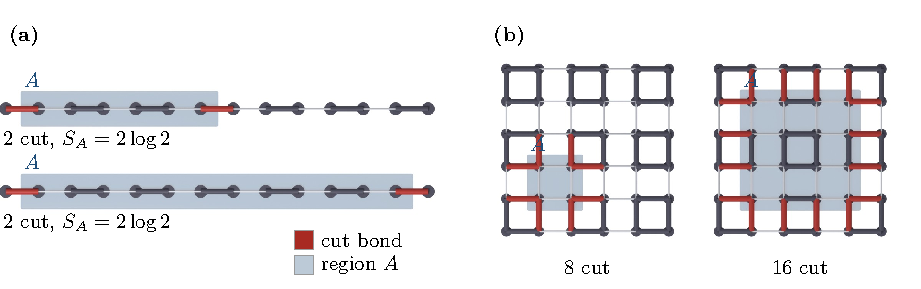
\includegraphics{figures/pdf/s07f02_arealaw.pdf}
\end{aqmfigure}


This behavior is called the \textbf{area law}. For the ground state of a gapped and local Hamiltonian,
the entanglement entropy of a subsystem scales with the size of the boundary between the subsystem
and the rest of the system, which is a fixed number of points in 1D, a length in 2D and an area in 3D,

\begin{equation}
S_A \;\sim\; \alpha\, |\partial A|,
\end{equation}

and not with the \emph{volume} of $A$. This is a strong restriction. A random state taken uniformly
from the full Hilbert space of dimension $2^L$ would usually have $S_A$ close to its maximum value,
which is $|A|\log 2$ for a spin-1/2 subsystem of size $|A|$, and this is called a volume law. In this
sense, gapped ground states are very far from typical states. They live only in the very small part
of the Hilbert space that satisfies the area law. The dimer and tetramer models above are exactly in
this part, and realistic gapped Hamiltonians are approximately in it.

\section{Why MPS work in 1D, and where they stop working}

The area law is the missing piece that explains why the ansatz (7.5) is a good one. Let us take an
MPS at a given bond, and use it to build the Schmidt decomposition of the state for a division of the
system at that bond.

\begin{equation*}
|\Psi\rangle = \sum_{\alpha=1}^{M} \lambda_\alpha\, |\alpha\rangle_A \otimes |\alpha\rangle_B,
\end{equation*}

This sum has at most $M$ terms, because the internal index, also called virtual index, that runs
through that bond only takes $M$ values. Therefore the reduced density matrix $\rho_A = \sum_\alpha
\lambda_\alpha^2 |\alpha\rangle_A
\langle\alpha|_A$ has rank at most $M$. Among all density matrices with rank $\le M$, the
entropy (7.6) is maximal when all the eigenvalues are equal, $\lambda_\alpha^2 = 1/M$, which gives

\begin{equation}
S \;\le\; \log M.
\end{equation}

In other words, an MPS with bond dimension $M$ can have an entanglement entropy of at most $\log M$
across any bond, which grows only logarithmically with $M$. Let us compare this with (7.9). A 1D
gapped ground state has an entanglement entropy that \emph{saturates} at a finite value, which does
not depend on the size of the subsystem, so a moderate and fixed bond dimension is already enough to
describe it almost exactly. This is the precise and quantitative reason why matrix product states are
such a good ansatz in one dimension, since the area law limits the same quantity that the bond
dimension limits. Geometrically, we can think of the full many-body Hilbert space as a large set, and
MPS describe only a very small part of it, which is the part of area-law states. This part is reached
with a bond dimension that stays moderate ($M \sim 10$, $100$) as long as we stay in the area-law
regime. To reach a general state with a volume law, the bond dimension would have to become very
large, $M \sim 2^{L/2}$, which is exponential in $L$. Figure~\ref{fig:s07:ceiling} shows this comparison directly. It
shows the upper limit
$\log M$ given by (7.10) and the entropy that a gapped, a critical and a general state
need when the subsystem grows.

% Session 7 -- what an MPS of bond dimension M can and cannot represent.
% Placement: sec. "Why MPS work in 1D, and where they stop working", after (7.10).
%
% LAYOUT NOTE: the only pgfplots figure of this set. Everything, annotations
% included, is positioned in (axis cs:...) so nothing can drift off the curves.
\begin{aqmfigure}{fig:s07:ceiling}{The bond dimension is an upper limit on the entanglement, and this
determines when matrix product states work. An MPS with bond dimension $M$ has at most $M$
Schmidt terms across any bond, so by (7.10) it can have at most $S=\log M$ there, which is shown by
the two horizontal lines. A gapped one-dimensional ground state follows the area law of Section 7.6,
and its entropy saturates at a value set by the correlation length and not by the subsystem size, so
it stays below a fixed and moderate limit for any chain length. A critical chain violates the area law
logarithmically, (7.12), so it goes above any fixed limit at some point, and $M$ must be increased as
the system grows, slowly but without bound. A general state of the Hilbert space of dimension $2^L$
follows a volume law, $S=\ell\log 2$, and it goes above any usable $M$ after a few sites. This is why
time evolution over long times, highly excited states and two-dimensional systems are all out of
reach. The entropy is drawn in bits, $S/\log 2$, with central charge $c=1$, and the curves are
schematic and not fits to a specific model.}

\begin{tikzpicture}
\begin{axis}[
  aqmplot,
  width=12.4cm, height=7.0cm,
  axis lines=left,
  axis line style={aqm, black},
  xlabel={subsystem size $\ell$ (sites)},
  ylabel={$S/\log 2$},
  xlabel style={at={(axis description cs:0.5,-0.11)}, anchor=north},
  ylabel style={at={(axis description cs:-0.075,0.5)}, anchor=south, rotate=90},
  xmin=0, xmax=74, ymin=0, ymax=6.5,
  xtick={0,16,32,48,64}, ytick={0,2,4,6},
  enlargelimits=false,
]

% --- the two MPS ceilings, S = log M ----------------------------------------
\addplot[aqmguide, forget plot, domain=0:74, samples=2] {2};
\addplot[aqmguide, forget plot, domain=0:74, samples=2] {4};
\node[aqmlabsmall, anchor=south west, text=aqmmuted] at (axis cs:6.5,2.04)
  {$\log M$ for $M=4$};
\node[aqmlabsmall, anchor=south west, text=aqmmuted] at (axis cs:6.5,4.04)
  {MPS ceiling $S=\log M$, $\;M=16$};

% --- volume law: a generic state --------------------------------------------
\addplot[aqmcurvebroken, dash pattern=on 4pt off 2pt, domain=0:6.4, samples=2] {x};
\node[aqmlabsmall, anchor=west, align=left, text=aqmbroken] at (axis cs:7.6,5.62)
  {generic (volume-law) state: $S=\ell\log 2$\\[-1pt]
   no practical $M$ survives past a few sites};

% --- critical 1D chain: (c/3) log l ------------------------------------------
\addplot[black, smooth, dash pattern=on 2.5pt off 2pt, domain=1:74, samples=120]
  {0.4809*ln(x)+0.35};
\node[aqmlabsmall, anchor=north east, align=right] at (axis cs:73,1.92)
  {critical 1D chain, $S=\frac{c}{3}\log\ell$ (7.12):\\[-1pt]
   grows without bound, so $M$ must grow too};

% --- gapped 1D ground state: saturates ---------------------------------------
\addplot[aqmcurve, domain=0:74, samples=140] {0.90*(1-exp(-x/3.2))};
\node[aqmlabsmall, anchor=north west, align=left, text=aqmaccent] at (axis cs:26,0.71)
  {gapped 1D ground state: $S$ saturates};

% --- where the small ceiling is exhausted ------------------------------------
\node[circle, draw=black, fill=white, line width=\aqmthinwidth, minimum size=5pt,
      inner sep=0pt] (xcross) at (axis cs:30.9,2) {};
\draw[aqmguide, draw=aqmmuted] (axis cs:30.9,2.78) -- (xcross);
\node[aqmlabsmall, anchor=north west, align=left] at (axis cs:19,3.52)
  {$M=4$ is exhausted here; a larger $M$ lifts the\\[-1pt]
   ceiling, but it never flattens the curve};

\end{axis}
\end{tikzpicture}

\end{aqmfigure}


The same argument tells us directly where MPS must fail, which is whenever the true entanglement
entropy is larger than what a practical bond dimension can give through (7.10). In practice this
happens in four cases. The first case is dynamics over long times, since after a quench the
entanglement grows \emph{linearly} with time and not logarithmically. The second case is systems in
more than one dimension, where the length of the boundary in the area law grows with the system size,
as we saw in Section 7.7, so $M$ has to grow too, often exponentially in the linear size of the
subsystem. The third case is highly excited states, since the area law is a statement about ground
states and not about general eigenstates. The fourth case is, more generally, states far from
equilibrium. However, when the physics stays close to a gapped 1D ground state, MPS can be used for
more than the ground-state problem. With a higher cost, they can be used for time evolution, excited
states and open quantum systems, routinely in 1D and in some cases in 2D.

\begin{notebookbox}{\texttt{session7.ipynb}, ``Near linear scaling with system size with matrix product states'' (Core) and ``The role of the bond dimension in tensor networks'' (Core)}
In the first exercise you check directly that the cost of the DMRG ground-state calculation in
\texttt{dmrgpy} grows linearly with the system size, which is the $L\times M^2$ scaling of (7.5) and
not the $2^L$ scaling of (7.4). In the second exercise you change the bond dimension and see how the
fluctuation of the ground-state energy becomes smaller and then saturates. The point where it
saturates is where $M$ is large enough to satisfy the bound (7.10) for that state.
\end{notebookbox}

\begin{notebookbox}{\texttt{session7.ipynb}, ``Entanglement entropy of the ground state'' (Core), ``Size dependence of the entanglement entropy'' (Challenge), and ``Bond dimension dependence of the entanglement entropy'' (Challenge)}
With these three exercises you can reproduce Sections 7.5 to 7.8 numerically. First, you compute the
entanglement entropy at each bond for the MPS ground state of a Heisenberg chain. Then you check that
it grows very little with the system size, which is the 1D area-law saturation of Section 7.6, but
this time in a gapless chain and not in a gapped one. Finally, you check that it saturates once the
bond dimension is large enough to satisfy (7.10). The quiz of the first exercise also asks you to
replace the model with an Ising model and to see how the entropy changes. This is a quick way to see
how the area law responds to a really different ground state, which in this case is classical and has
zero entanglement.
\end{notebookbox}

\section{Tensor diagrams as notation for networks and operators}

Matrix product states come with a convenient graphical notation, which makes it much easier to think
about both the ansatz and the algorithms built on it. A scalar, which is a tensor of rank 0, is drawn
as a point. A vector, of rank 1, is a point with one free leg. A matrix, of rank 2, is a point with two
legs. A tensor of rank 3 is a point with three legs, and so on for any rank. Each leg represents one
index of the tensor, and when we join two legs of two tensors, this means that we sum over the shared
index, which is called a contraction.

An MPS is then a horizontal chain of such points, with one point per site. Each point has one
\emph{physical} leg pointing down, which is the index $s_i$, the local spin value. It also has one or
two \emph{virtual} legs that connect it to its neighbors in the chain, and these carry the
bond-dimension index that is summed over. A \textbf{matrix product operator} (MPO) represents an
operator, in particular the Hamiltonian, in the same way. Now each site has \emph{two} physical
legs instead of one, which correspond to the two indices $\sigma_i,\sigma_i'$ of the operator, and the
same virtual legs that link neighboring sites. To apply an MPO to an MPS, for example to compute
$H|\Psi\rangle$, we join the two diagrams along the physical legs and contract them. This means that
we multiply every pair of matrices that share an index and sum over that index. If we do this in a
naive way, the bond dimensions of the two objects are multiplied, which would remove the advantage of
the method. In practice, we do a singular value decomposition of the result and keep only the largest
singular values, so we truncate back to a bond dimension that we can handle, and we remove
the least important part of the Hilbert space that is represented. This truncation step is the
practical core of almost every MPS algorithm, including the ground-state search of the next section.
Figure~\ref{fig:s07:tensors} shows together the notation, the ansatz (7.5) drawn in this notation,
and this step of contraction and truncation.

% Session 7 -- tensor diagram notation, the MPS, and the MPO/truncation step.
% Placement: sec. "Tensor diagrams: notation for networks and operators", after the
% Rendered by figures/blender/s07f04_tensordiagram.py, labels in figures/overlays/s07f04_tensordiagram.tex.
\begin{aqmfigure}{fig:s07:tensors}{The graphical notation, and the MPS ansatz drawn in it. (a) A
tensor is a block and each of its indices is a leg, so a scalar has no leg, a vector has one leg, a
matrix has two, and so on. Joining two legs means summing over the shared index. (b) The exact
coefficient tensor of (7.4) is a single object with one leg per site, and it contains $2^L$
independent numbers. The matrix product state (7.5) replaces it with a chain of small tensors. Each
of them has one physical leg pointing down and virtual legs of dimension $M$ that link it to its
neighbours, for a total of $\sim 2LM^2$ numbers, so the exponential growth is replaced by a chain
that grows linearly. (c) An operator, in particular the Hamiltonian, becomes a matrix product
operator, the darker row, with two physical legs per site. To apply it to a state we join the
diagrams along the shared physical legs and contract them, which multiplies the two bond dimensions.
A singular value decomposition that keeps only the largest singular values then truncates the result
back to a usable $M$. This truncation is the core of every MPS algorithm, including DMRG.}
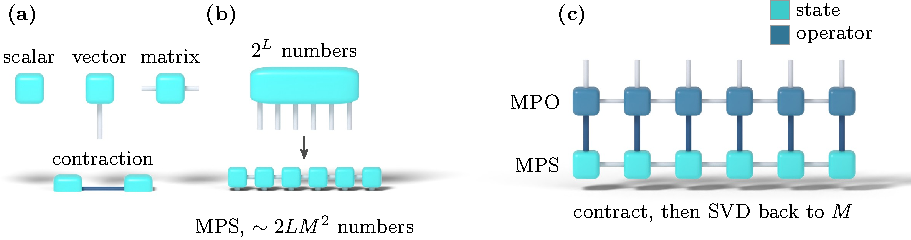
\includegraphics{figures/pdf/s07f04_tensordiagram.pdf}
\end{aqmfigure}


\section{The variational principle and DMRG for the ground state}

An ansatz is only useful if we can optimize it. We take the MPS matrices $\{M_i^{s_i}\}$ as
variational parameters and minimize the Rayleigh quotient

\begin{equation}
E[\Psi] = \frac{\langle \Psi | H | \Psi \rangle}{\langle \Psi | \Psi \rangle},
\end{equation}

or, in an equivalent way, we introduce a Lagrange multiplier $\lambda$ for the normalization and
minimize $\langle
\Psi|H|\Psi\rangle - \lambda\left(\langle\Psi|\Psi\rangle - 1\right)$ with respect to every matrix in
the network. In the diagrams, the derivative with respect to one tensor in the network, for example
the matrix at site $k$, corresponds to ``erasing'' that tensor from the diagram. The reason is that
each tensor appears once in the bra layer and once in the ket layer, so with the other tensors fixed
the energy is a quadratic form in that tensor, and it is linear in the bra copy alone. When we erase
the bra tensor of site $k$ from both the numerator and the denominator diagrams, what is left is a
generalized eigenvalue problem for that single tensor, which becomes an ordinary one when the other
tensors are chosen orthonormal. It involves an effective, reduced Hamiltonian that acts on the
indices of site $k$, and its ground eigenvector is the locally optimal
replacement for $M_k^{s_k}$. Figure~\ref{fig:s07:dmrg} shows this erasure and the sweep that follows
from it.

% Session 7 -- DMRG: differentiating the network erases one tensor and leaves a
% small eigenvalue problem; sweeping that problem along the chain is the algorithm.
% Placement: sec. "Finding the ground state: the variational principle and DMRG",
% after the "erasing that tensor from the diagram" paragraph.
%
% LAYOUT NOTE: pure TikZ, canvas coordinates; one-off tensor styles are \tikzset
% inside this picture only. Panel titles are short tags, with the explanatory line
% placed under each panel, so nothing collides across the top of the figure.
\begin{aqmfigure}{fig:s07:dmrg}{How DMRG turns an exponentially large minimization into a sequence of
small ones. (a) The numerator of the Rayleigh quotient (7.11) is a single closed network, made of the
ket MPS, the Hamiltonian as an MPO and the bra MPS, all contracted together. It has no free legs, so
it is a number. (b) Every tensor enters that network once in the bra layer and once in the ket layer, so
the energy is a quadratic form in each tensor and linear in its bra copy, and the derivative with
respect to the bra tensor at site $k$ removes it. What is left has
exactly three open legs, the two virtual bonds and the physical index of site $k$, which are the
indices of the tensor $M_k^{s_k}$ that we want to find. Everything to the left and right of $k$ has
been reduced to an environment, and the stationarity condition is a generalized eigenvalue problem,
which is an ordinary one in an orthonormal gauge, with the size of a single tensor. (c) We solve it, move one site along, solve again, and sweep back and
forth until the energy stops decreasing. This is the density matrix renormalization group, and at no
point do we build an object of size $2^L$.}

\begin{tikzpicture}[x=1cm, y=1cm]
\tikzset{
  tens/.style={aqm, circle, draw=black, fill=aqmfill, minimum size=6.5pt, inner sep=0pt},
  tensop/.style={aqm, rectangle, draw=black, fill=white, minimum size=6.5pt, inner sep=0pt},
  leg/.style={aqm, draw=black, line width=\aqmthinwidth},
  openleg/.style={aqm, draw=aqmbroken, line width=1.15pt}
}

% ============================ (a) the closed network ========================
\node[aqmpanel, anchor=west] at (-0.05,0.60) {(a)};

\node[aqmlabsmall, anchor=east] at (0.42,0.10)  {$\langle\Psi|$};
\node[aqmlabsmall, anchor=east] at (0.42,-0.52) {$H$};
\node[aqmlabsmall, anchor=east] at (0.42,-1.14) {$|\Psi\rangle$};

\foreach \i in {0,1,2,3,4} {
  \node[tens]   (b\i) at (0.62+0.58*\i, 0.10)  {};
  \node[tensop] (h\i) at (0.62+0.58*\i,-0.52)  {};
  \node[tens]   (k\i) at (0.62+0.58*\i,-1.14)  {};
  \draw[leg] (b\i) -- (h\i);
  \draw[leg] (h\i) -- (k\i);
}
\foreach \i/\j in {0/1, 1/2, 2/3, 3/4} {
  \draw[leg] (b\i) -- (b\j);
  \draw[leg] (h\i) -- (h\j);
  \draw[leg] (k\i) -- (k\j);
}
\node[aqmlabsmall, anchor=north, text=aqmmuted, align=center] at (1.78,-1.44)
  {$\langle\Psi|H|\Psi\rangle$: no free legs,\\[-1pt] so the contraction is a number};

% ============================ the differentiation arrow =====================
\draw[aqmarrowaccent] (3.40,-0.52) -- (4.92,-0.52);
\node[aqmlabsmall, anchor=south, align=center, text=aqmaccent] at (4.15,-0.44)
  {erase the bra\\[-1pt] tensor at $k$};

% ============================ (b) the hole ==================================
\node[aqmpanel, anchor=west] at (5.25,0.60) {(b)};

\foreach \i in {0,1,2,3,4} {
  \node[tensop] (H\i) at (5.65+0.58*\i,-0.52)  {};
  \node[tens]   (K\i) at (5.65+0.58*\i,-1.14)  {};
  \draw[leg] (H\i) -- (K\i);
}
\foreach \i in {0,1,3,4} {
  \node[tens] (B\i) at (5.65+0.58*\i, 0.10)  {};
  \draw[leg] (B\i) -- (H\i);
}
\foreach \i/\j in {0/1, 1/2, 2/3, 3/4} {
  \draw[leg] (H\i) -- (H\j);
  \draw[leg] (K\i) -- (K\j);
}
% the hole at site k, and the three legs it leaves open
\draw[openleg] (B1) -- (6.60,0.10);
\draw[openleg] (7.00,0.10) -- (B3);
\draw[openleg] (H2) -- (6.80,-0.12);
\node[circle, draw=aqmbroken, dashed, line width=\aqmthinwidth, fill=none,
      minimum size=12pt, inner sep=0pt] at (6.80,0.10) {};
\node[aqmlabsmall, anchor=south, align=center, text=aqmbroken] at (6.80,0.34)
  {site $k$ erased};
\node[aqmlabsmall, anchor=north, text=aqmbroken, align=center] at (6.80,-1.44)
  {three open legs: exactly the\\[-1pt] indices of one tensor $M_k^{s_k}$};

\node[aqmboxaccent, anchor=west, text width=4.5cm, align=center] at (8.75,-0.52)
  {$H^{\text{eff}}_k\,M_k^{s_k} = \lambda\,M_k^{s_k}$\\[3pt]
   {\footnotesize\textcolor{aqmmuted}{one small eigenvalue problem; the rest of the chain is
   now just an environment}}};

% ============================ (c) the sweep =================================
\node[aqmpanel, anchor=west] at (-0.05,-2.48) {(c)};

\foreach \i in {0,...,7} {
  \node[tens] (s\i) at (0.62+0.58*\i,-3.20) {};
  \draw[leg] (0.62+0.58*\i,-3.28) -- (0.62+0.58*\i,-3.52);
}
\foreach \i/\j in {0/1, 1/2, 2/3, 3/4, 4/5, 5/6, 6/7} { \draw[leg] (s\i) -- (s\j); }

\draw[aqmarrowaccent] (0.50,-2.86) -- (4.82,-2.86);
\node[aqmlabsmall, anchor=west, text=aqmaccent] at (5.05,-2.86)
  {solve one tensor, move one site along};
\draw[aqmarrowmuted] (4.82,-3.78) -- (0.50,-3.78);
\node[aqmlabsmall, anchor=west, text=aqmmuted] at (5.05,-3.78)
  {\dots{} then sweep back, until the energy stops decreasing};

\end{tikzpicture}

\end{aqmfigure}


This suggests an iterative algorithm. We fix every tensor except the
one of site $1$, solve the local eigenvalue problem there, and update $M_1^{s_1}$ with the resulting
eigenvector. Then we move to site $2$, fix everything else, solve the local eigenvalue problem there,
and update. We continue sweeping through the chain, site by site, until the energy stops decreasing.
This sweeping procedure is the \textbf{density matrix renormalization group (DMRG)} algorithm. Its
efficiency comes from the property of (7.11) that we used to build it. At every step we optimize only
one matrix at a time, which is a small linear-algebra problem that we can solve, instead of searching
for the ground state in the full exponentially large space at once.

\begin{notebookbox}{\texttt{session7.ipynb}, ``Low energy excitations of a Heisenberg model'' (Core)}
In this exercise you look at the matrix elements between the DMRG ground state and the first excited
state of a Heisenberg chain, meaning what the sweeping procedure of Section 7.10 finds one level above
the state that directly minimizes (7.11).
\end{notebookbox}

\section{MERA and PEPS beyond MPS}

Matrix product states are the simplest member of a much larger family, which is called \textbf{tensor
networks}. Nothing requires the tensors to sit in a 1D chain, and the same coefficient tensor $C$
of (7.4) can also be drawn as a 2D grid or as a general graph of connections. A richer connectivity
makes the optimization harder, and MPS are the tensor network that is easiest to optimize, but in
exchange it can represent a larger class of states. Let us mention two of these architectures.

The \textbf{multi-scale entanglement renormalization ansatz (MERA)} organizes its tensors in a
hierarchy of length scales instead of along a single chain. This extra structure allows it to
describe more entanglement than an MPS with a comparable number of parameters. This is important
because the area law (7.9) is strictly a statement about \emph{gapped} systems. At a critical point,
which is a continuous quantum phase transition usually described by a conformal field theory in 1+1
dimensions, the entanglement entropy of the ground state does not saturate anymore. Instead, it grows
logarithmically with the size of the subsystem,

\begin{equation}
S(\ell) \;=\; \frac{c}{3}\log \ell \;+\; \text{const.},
\end{equation}

where $c$ is the central charge of the CFT. This is a weak but real violation of the strict area
law (7.9), and the extra hierarchical structure of MERA is built to describe this kind of weak
violation. For this reason MERA is the tensor network that is used at criticality.

\textbf{Projected entangled pair states (PEPS)} are the direct 2D generalization of the MPS idea.
Instead of tensors coupled in a line, the tensors sit on the nodes of a real 2D lattice, and they are
coupled to all their lattice neighbors. This is a natural and promising architecture for 2D quantum
many-body problems, but it has a real cost. For PEPS there is no analogue of the simple local
eigenvalue problem for a single tensor that we have in DMRG, because the contraction of a general 2D
tensor network is itself a hard computational problem. This is different from the 1D contraction,
which is what made the local eigenvalue problem of Section 7.10 possible to solve. The optimization of
PEPS is still an open and harder problem. Figure~\ref{fig:s07:merapeps} shows both architectures,
where the extra structure of each one comes from and what it costs.

% Session 7 -- MERA and PEPS: the two architectures the section names but never draws.
% Placement: sec. "Beyond MPS: MERA and PEPS", after the PEPS paragraph.
%
% LAYOUT NOTE: pure TikZ, canvas coordinates; one-off tensor shapes declared with
% \tikzset inside this picture only.
\begin{aqmfigure}{fig:s07:merapeps}{The two tensor networks beyond the chain, and what their geometry
buys. Left: the multi-scale entanglement renormalization ansatz. Its tensors are stacked in layers,
each layer first removing the short-range entanglement between neighbouring blocks (the square
disentanglers) and then coarse-graining two sites into one (the triangular isometries), so that the
network describes the state at successively longer length scales rather than at successive positions
along a chain. A bipartition now cuts one bond in every layer instead of one bond in total, which is
precisely how MERA supports the logarithmically growing entropy (7.12) of a critical chain that an
MPS of fixed bond dimension cannot reach. Right: projected entangled pair states, the honest 2D
generalization of (7.5), with one tensor per lattice site carrying a physical leg and four virtual
bonds. The picture also shows the difficulty: there is no way to sweep along such a network one
tensor at a time with the rest reduced to a simple environment, and contracting it exactly is itself
a hard problem, which is why PEPS has no clean analogue of DMRG.}

\begin{tikzpicture}[x=1cm, y=1cm]
\tikzset{
  tens/.style={aqm, circle, draw=black, fill=aqmfill, minimum size=6.5pt, inner sep=0pt},
  diseng/.style={aqm, rectangle, draw=black, fill=white, minimum size=8pt, inner sep=0pt},
  isom/.style={aqm, regular polygon, regular polygon sides=3, draw=black, fill=aqmfill,
               minimum size=11pt, inner sep=0pt},
  leg/.style={aqm, draw=black, line width=\aqmthinwidth}
}

% ============================ (a) MERA ======================================
\node[aqmpanel, anchor=west] at (-0.10,3.30) {(a) MERA: layers across length scales};

% --- physical sites -----------------------------------------------------------
\foreach \i in {0,...,7} {
  \node[tens] (p\i) at (0.42*\i,0) {};
  \draw[leg] (0.42*\i,-0.08) -- (0.42*\i,-0.34);
}

% --- layer 1: disentanglers on (1,2), (3,4), (5,6) ---------------------------
\foreach \c/\l/\r in {0.63/1/2, 1.47/3/4, 2.31/5/6} {
  \node[diseng] (u\l) at (\c,0.62) {};
  \draw[leg] (p\l) -- (u\l);
  \draw[leg] (p\r) -- (u\l);
}
% --- layer 1: isometries on (0,1), (2,3), (4,5), (6,7) -----------------------
\foreach \c/\n in {0.21/0, 1.05/1, 1.89/2, 2.73/3} {
  \node[isom] (w\n) at (\c,1.32) {};
}
\draw[leg] (p0) -- (w0);
\draw[leg] (u1) -- (w0);
\draw[leg] (u1) -- (w1);
\draw[leg] (u3) -- (w1);
\draw[leg] (u3) -- (w2);
\draw[leg] (u5) -- (w2);
\draw[leg] (u5) -- (w3);
\draw[leg] (p7) -- (w3);

% --- layer 2 -----------------------------------------------------------------
\node[diseng] (uu) at (1.47,1.92) {};
\draw[leg] (w1) -- (uu);
\draw[leg] (w2) -- (uu);
\node[isom] (v0) at (0.63,2.56) {};
\node[isom] (v1) at (2.31,2.56) {};
\draw[leg] (w0) -- (v0);
\draw[leg] (uu) -- (v0);
\draw[leg] (uu) -- (v1);
\draw[leg] (w3) -- (v1);
\node[tens] (top) at (1.47,3.02) {};
\draw[leg] (v0) -- (top);
\draw[leg] (v1) -- (top);

% --- the scale axis ----------------------------------------------------------
\draw[aqmarrowmuted] (-0.62,-0.20) -- (-0.62,3.00);
\node[aqmlabmuted, rotate=90, anchor=south] at (-0.76,1.40) {coarser length scale};

% --- legend and message ------------------------------------------------------
\node[diseng] at (3.75,0.62) {};
\node[aqmlabsmall, anchor=west] at (3.92,0.62) {disentangler};
\node[isom] at (3.75,1.32) {};
\node[aqmlabsmall, anchor=west] at (3.92,1.32) {isometry ($2\to1$ sites)};
\node[aqmlabsmall, anchor=west, align=left, text width=3.3cm, text=aqmaccent] at (3.65,2.45)
  {a bipartition cuts one bond \emph{per layer}, so $S$ can grow like $\log\ell$: the critical
   law (7.12)};
\node[aqmlabsmall, anchor=north, text=aqmmuted] at (1.47,-0.48) {physical legs};

% ============================ (b) PEPS ======================================
\node[aqmpanel, anchor=west] at (7.30,3.30) {(b) PEPS: a 2D grid of tensors};

\begin{scope}[shift={(8.20,0.85)}]
  \foreach \i in {0,1,2,3} { \foreach \j in {0,1,2,3} {
      \node[tens] (t\i\j) at (0.62*\i,0.62*\j) {};
      \draw[leg] (0.62*\i-0.05,0.62*\j-0.05) -- (0.62*\i-0.24,0.62*\j-0.24);
  }}
  \foreach \i/\k in {0/1, 1/2, 2/3} { \foreach \j in {0,1,2,3} {
      \draw[leg] (t\i\j) -- (t\k\j);
      \draw[leg] (t\j\i) -- (t\j\k);
  }}
\end{scope}
\node[aqmlabsmall, anchor=north, align=center, text width=4.4cm, text=aqmmuted] at (9.13,0.44)
  {four virtual bonds and one physical leg per site};
\node[aqmlabsmall, anchor=north, align=center, text width=4.4cm, text=aqmbroken] at (9.13,-0.34)
  {no 1D order to sweep along, and contracting the network is itself hard: DMRG's local
   eigenproblem has no analogue here};

\end{tikzpicture}

\end{aqmfigure}


This is also where the lecture of this year ends. In contrast with some previous editions of this
course, the recording of this year stops after MERA and PEPS, and it does not continue with neural
network quantum states. The single mention in Section 7.3 is all that we say about this topic in this
session. The tensor-network methods built in Sections 7.4 to 7.11 are still important,
since in session 10 we will use the same MPS, MERA and PEPS architectures directly as
machine-learning classifiers, and we will come back to neural network quantum states in detail, from
the point of view of machine learning.

\begin{notebookbox}{\texttt{session7.ipynb}, ``The entanglement entropy as a signal for phase transitions'' (Challenge)}
In this exercise you follow the entanglement entropy of the ground state of the transverse-field Ising
chain while you change the transverse field across its quantum critical point, using the MPS methods
of \texttt{dmrgpy}. Away from criticality you should see the area-law saturation of Section 7.8. Close
to the transition, you should see that the entropy does not saturate, as predicted by (7.12). The quiz
also asks which regime is the hardest for MPS, and this question asks you to connect back to the
reason why MERA exists.
\end{notebookbox}

\section{Closing summary}

\begin{itemize}
\item Strongly correlated matter, including quantum spin liquids and fractional Chern insulators, is
  the regime where the mean-field methods of sessions 1 to 6 have no order parameter to converge to,
  as we saw with (7.1) and in Section 7.1.
\item The \textbf{Jordan-Wigner transformation} (7.2) is an exact mapping between fermionic and
  spin-1/2 Hamiltonians, summarized as ``spin equals fermion times string.'' It is the link between
  the fermionic language of sessions 1-5 and the spin language of sessions 6 and 8, and it is the
  reason why we can work in the spin representation for the rest of the session.
\item The real obstruction to solving many-body Hamiltonians is \textbf{storage}, since a system of
  $L$ spins needs $2^L$ coefficients (7.4) to describe its wave function exactly.
\item The \textbf{matrix product state} ansatz (7.5) replaces these $2^L$ coefficients with $O(LM^2)$
  parameters, so we give up exactness in exchange for an approximation that we control with the bond
  dimension $M$.
\item The \textbf{entanglement entropy} (7.6), which we computed for the singlet in (7.7), measures how
  entangled a state is. Exactly solvable dimer and tetramer models show that gapped ground states
  follow an \textbf{area law} (7.9), with an entropy set by the length of the boundary and not by the
  volume of the subsystem.
\item The entanglement of an MPS is itself bounded, $S \le \log M$ (7.10). This is the reason why MPS
  work so well in 1D, where the area law saturates, and why they need an exponentially large $M$ in
  higher dimensions or away from the ground state.
\item Ground states are found variationally, by minimizing (7.11) one tensor at a time, and this
  sweeping procedure is the \textbf{DMRG} algorithm. \textbf{MERA} and \textbf{PEPS} extend the idea
  of tensor networks to criticality, through the logarithmic correction to the entropy (7.12), and to
  real 2D lattices, respectively. MERA can still be optimized tensor by tensor, while for PEPS the
  contraction is the hard step, so the simple local optimization of DMRG is lost.
\item Neural network quantum states were mentioned once, together with tensor networks, as a second
  answer to the same storage problem, but they were not developed in this session. In session 10 we
  will study them in detail from the point of view of machine learning, and we will also come back to
  the MPS, MERA and PEPS methods of this session as architectures for machine-learning classifiers.
\end{itemize}
